% !TeX root = ../paper_observer_consciousness.tex

Integrierte Information als Maß für das Bewusstsein zu verwenden ist Teil der \emph{Integratet Information Theory}
des Neurowissenschaftlers Giulio Tononi.\,\cite{Tononi_08} 
Die im Folgenden verwendete formale Definition für die Integrierte Information $\Phi$ weicht dabei von der 
Definition nach Tononi ab, ermöglicht aber ähnliche Aussagen. Die Integriert Information entspricht 
hier der minimalen Transinformation $I(\rho)$ die durch eine Trennung des Zustands $\rho$ in zwei Teilsystem
Zustände $\rho_{1}$ und $\rho_{2}$ erreicht werden kann.

\begin{empheq}{equation}
	\Phi = I_{\mathrm{min}} = \min I(\rho) = \min \del{S(\rho_1) + S(\rho_2) - S(\rho)}
\end{empheq}
Da ein Zustand mit $\Phi = I = 0$ in vollkommen unabhängige Teilzustände zerlegt werden kann und 
demnach möglichst unabhängigen Teilzustände die geringste Transinformation haben,  
wurde die Trennung des Zustands $\rho$  zur Bestimmung der Integrierten Information von Tononi
als \Quote{the cruelest cut} bezeichnet.

Eine mögliche Veranschaulichung von Integrierten Information ist das Speichern von Information mit 
unter Verwendung von Redundanz oder Fehlerkorrektur-Mechanismen. Dies findet beispielsweise in 
den weit verbreiteten QR-Codes Anwendung, deren Informationen nach Verlust eines Teils des Musters immer
noch zugänglich sind. Ein Beispiel dafür ist in \cref{fig:qrcode} dargestellt.
Durch numerische Berechnung kann die maximal mögliche Integration von Information eines Systems mit einer
festen Größe  von $n$ bit bestimmt werden. In  \cref{fig:maximal_integrated_information} ist dies beispielhaft 
für $n = \SI{14}{bit}$ gezeigt. Es ergibt sich, dass die maximal mögliche Integration für die Auswahl von 
{$\large \sfrac{n}{2}$} bit  zum speichern der Information vorliegt. Die übrigen {$\large \sfrac{n}{2}$} bit sorgen 
entsprechend für die notwendige Redundanz.


\begin{figure}
	\centering
	
\includegraphics[scale=0.15]{graphics/qrcode_damaged.jpg}
	\caption{Beispielhafte Darstellung eines QR-Code, dessen Information auch nach Entfernen von etwa 
		\SI{30}{\percent} des Musters noch nicht gelöscht ist.\label{fig:neuronqrcode}}
\end{figure}  
\begin{figure}
	\centering
	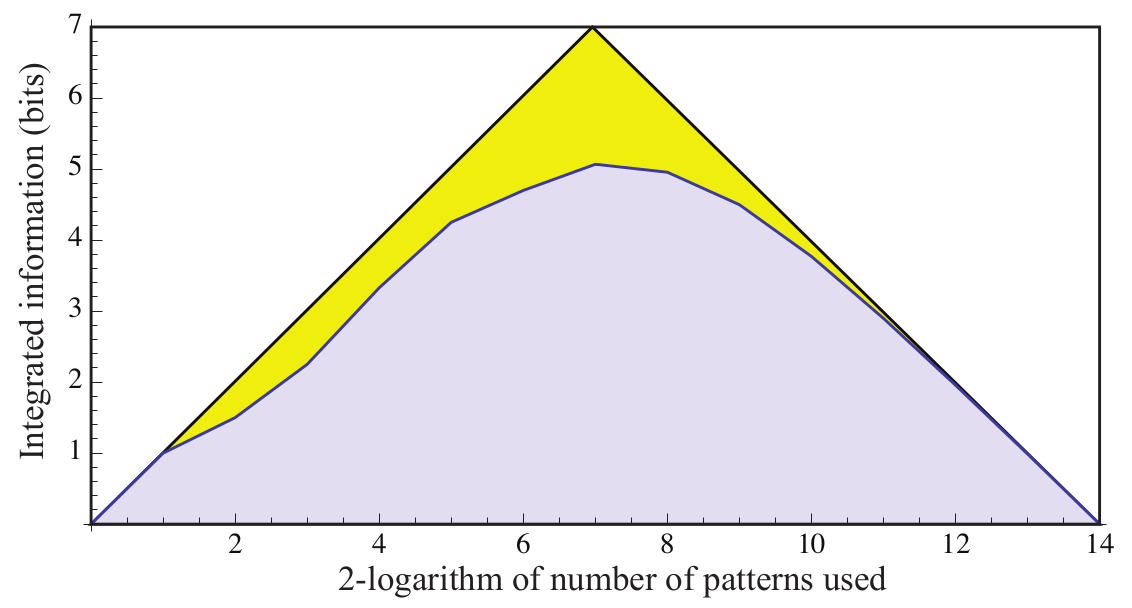
\includegraphics[scale=0.25]{graphics/integrated_information_graph.jpg}
	\caption{Darstellung der Ergebnisse der numerischen Suche nach maximaler Intgration in einem System 
		mit $n = \SI{14}{bit}$. Das Dreieck im Hintergrund stellt dabei die theoretisch maximal mögliche 
		Integration dar, die dem Minimum von Speicher-bits und Redundanz-bits entspricht. Die grau dargestellte
		Kurve gibt jeweils die maximale Integration für die jeweilige Anzahl an Speicher-bits an. \label{fig:maximal_integrated_information}}
\end{figure}  

Die Übertragung diese Konzepts in physikalische Systeme ist beispielsweise unter Betrachtung von 
\enquote{Eierkarton}-Potentiallandschaften, wie in \cref{fig:eggcrate_potential} dargestellt, möglich.
  




